In order to state the interaction between the different components of the system here are presented some sequence diagrams.
\\The sequence diagrams highlight the part of the system that interact for implement a function and the messages exchanged between them.


\begin{figure}[!ht]
  \centering
  \vspace{0.2cm}
  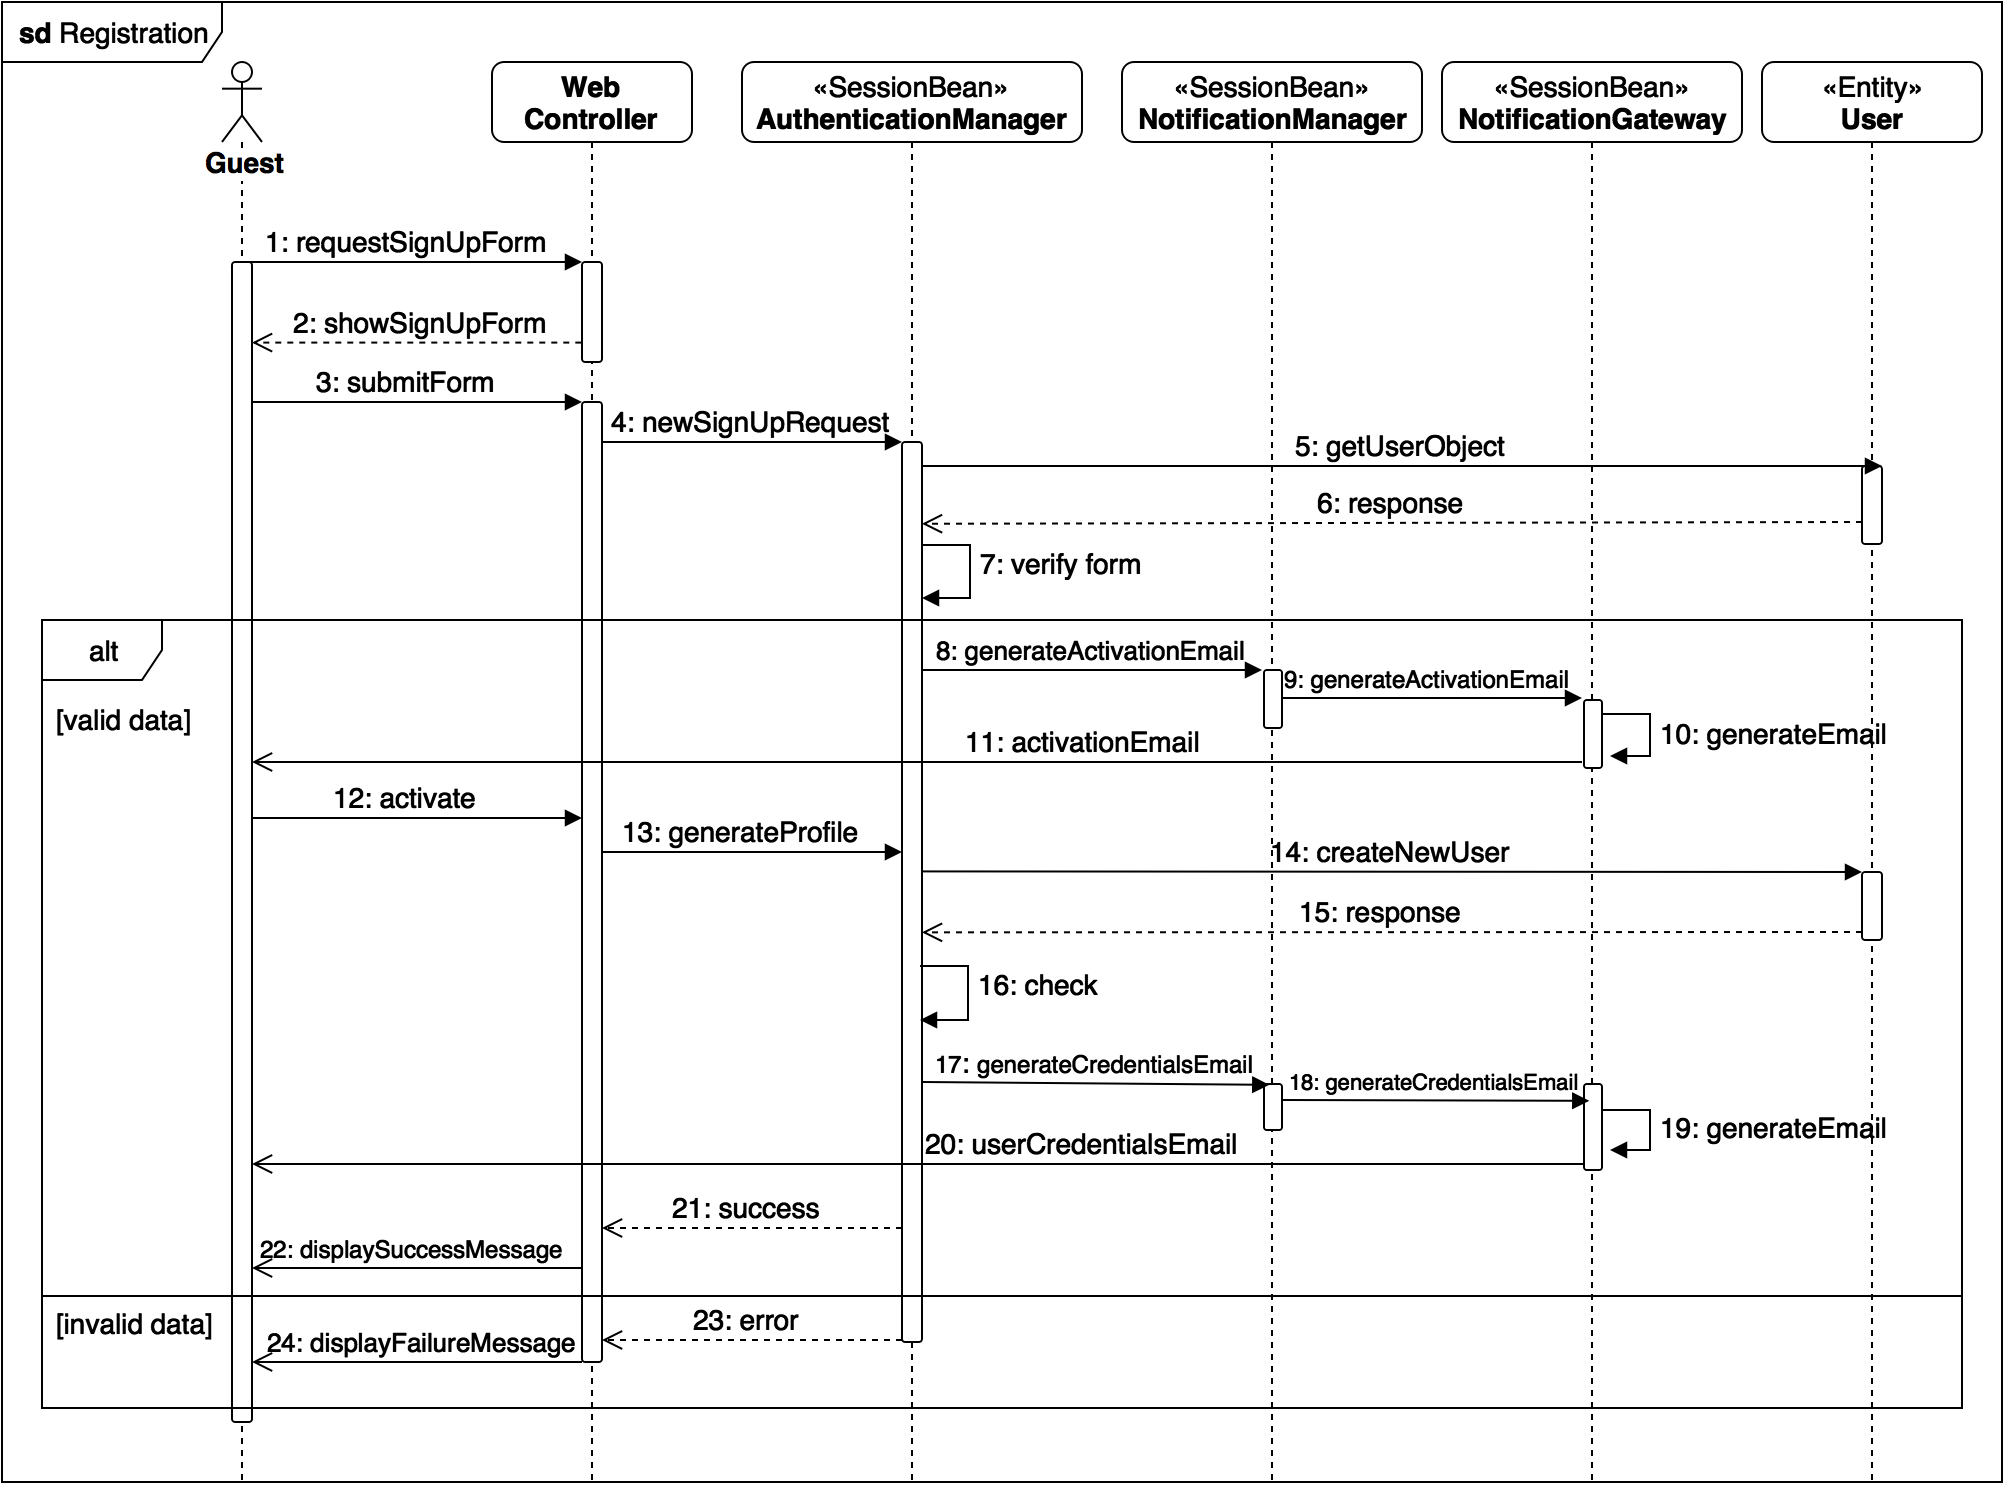
\includegraphics[width=1.0\textwidth]{/DD/Runtime_registration}\\
  \vspace{0.4cm}
  \caption{Registration sequence diagram: a new user sing up to PowerEnJoy using the Web application. } 
  \label{fig:Runtime_registration} 
\end{figure}
\newpage
\begin{figure}[!ht]
  \centering
  \vspace{0.2cm}
  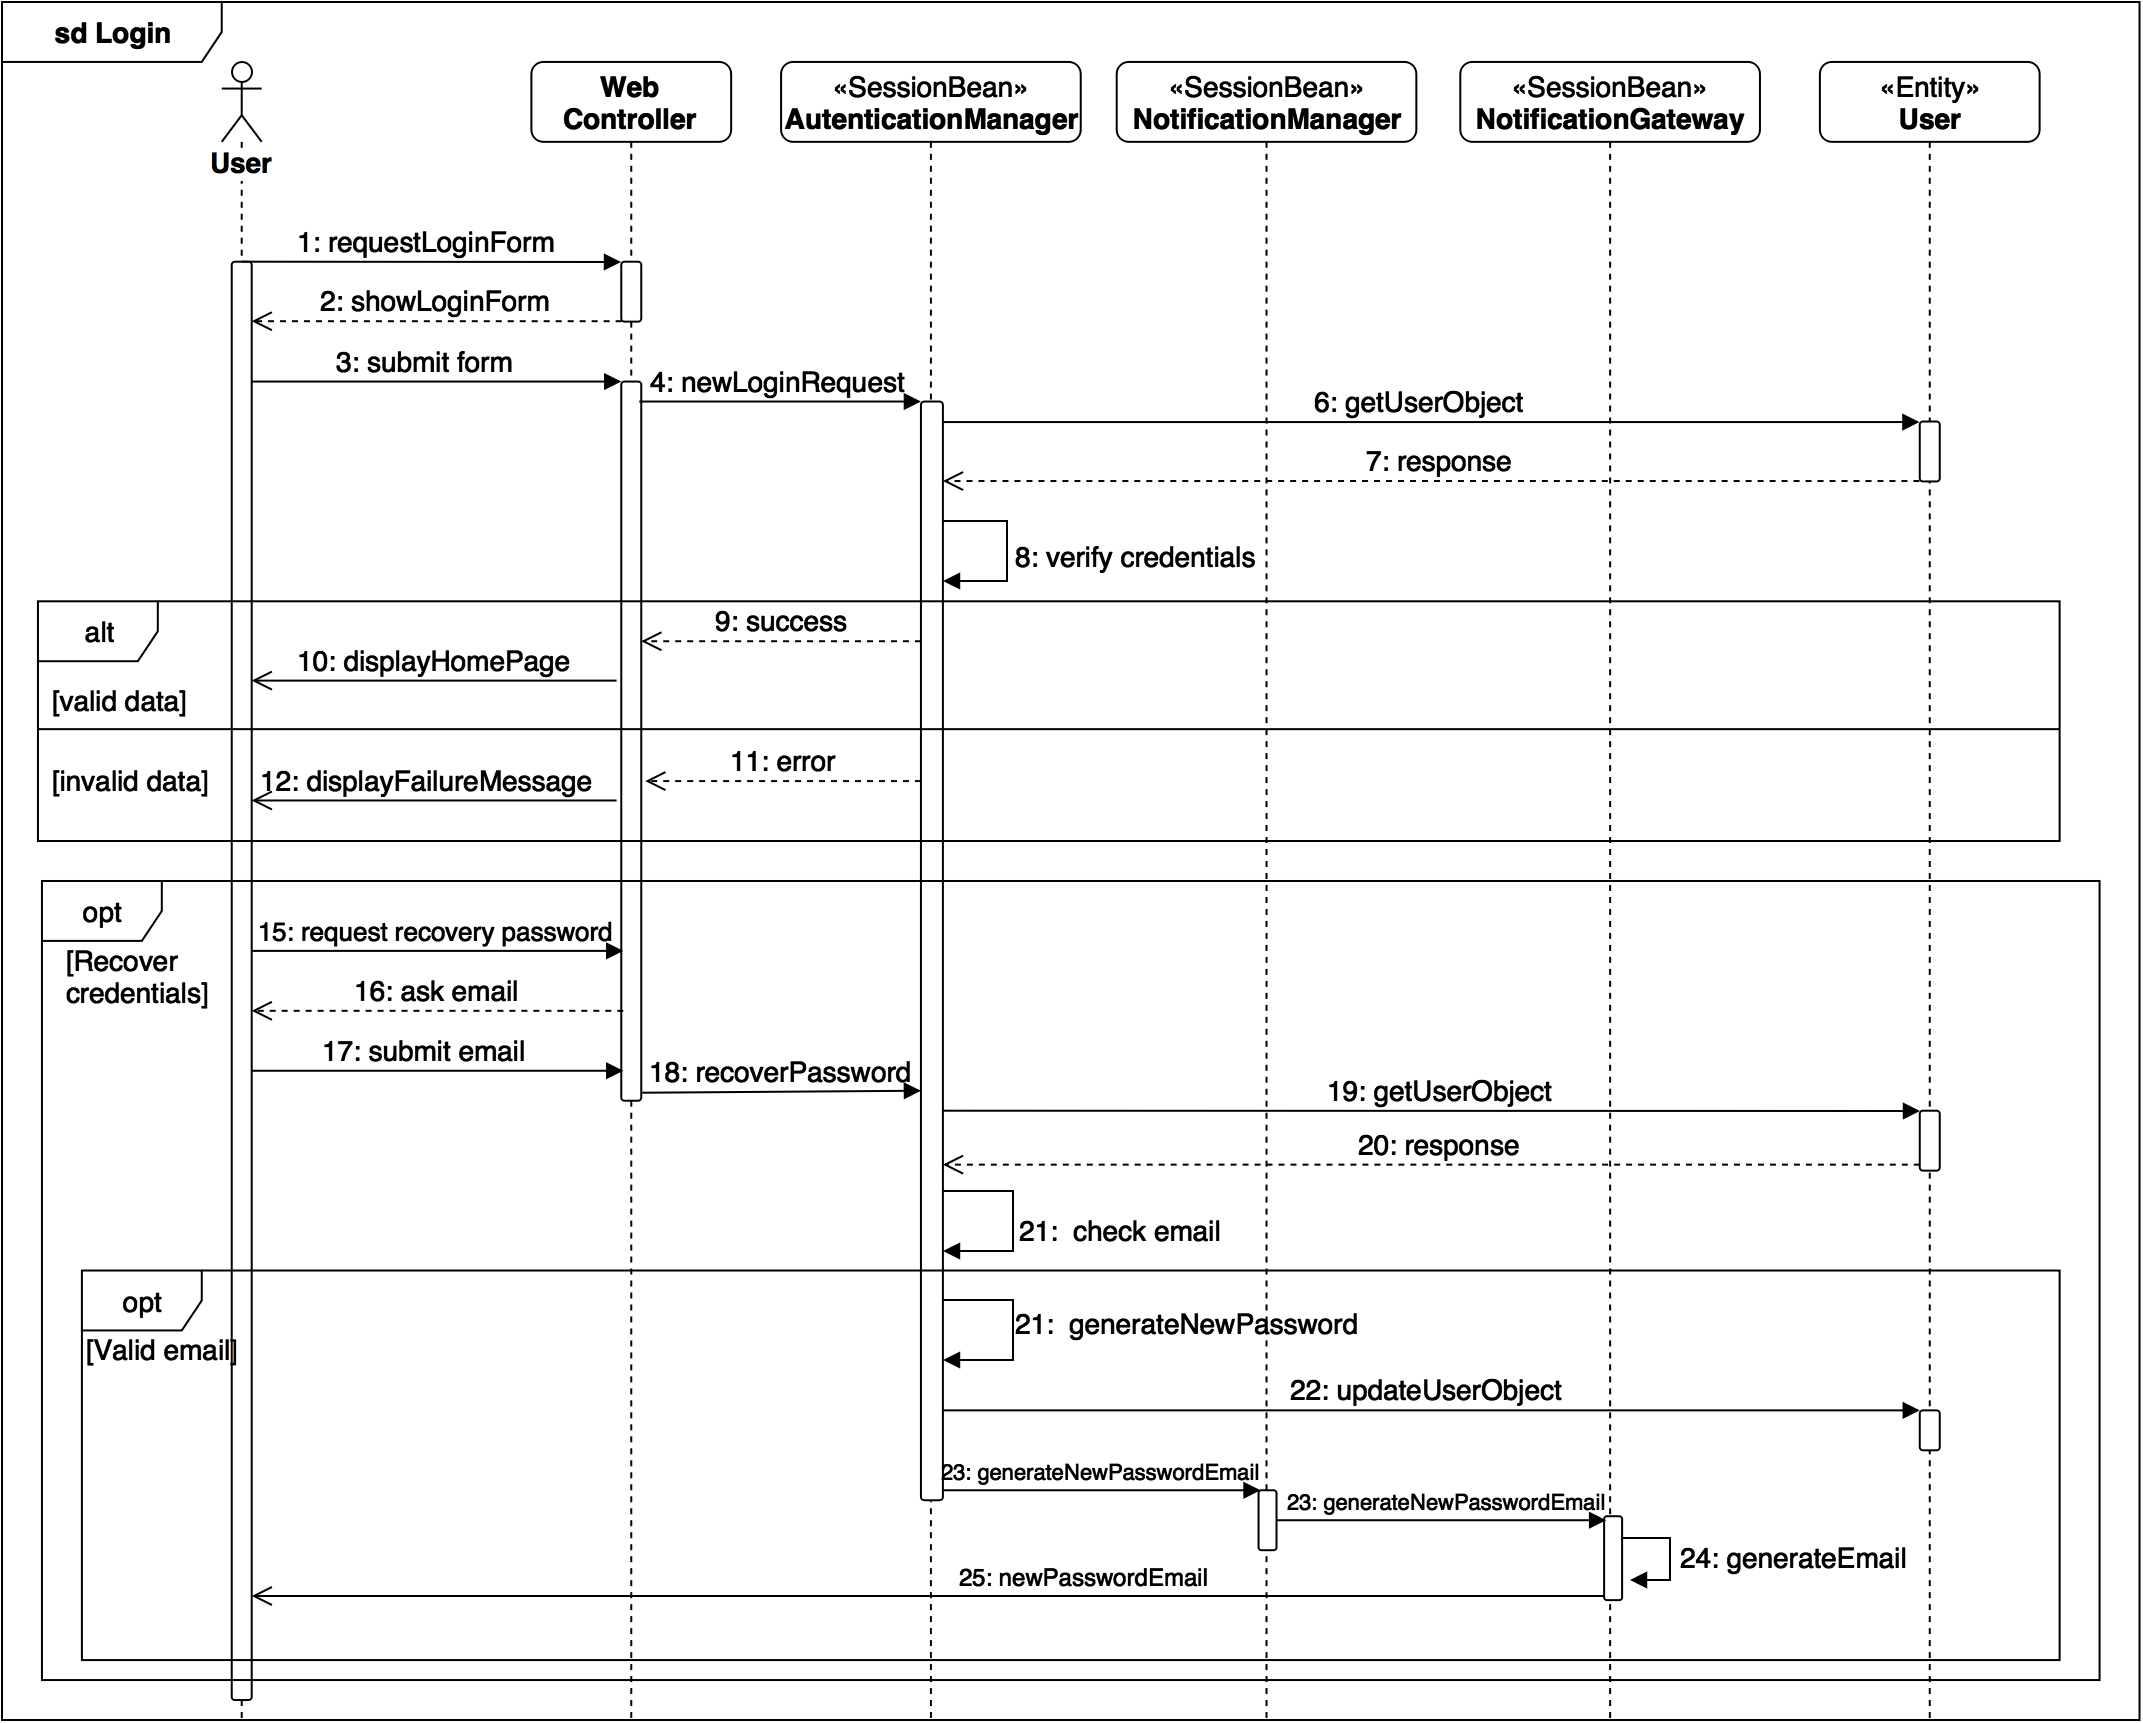
\includegraphics[width=1.0\textwidth]{/DD/Runtime_Login}\\
  \vspace{0.4cm}
  \caption{Login sequence diagram: an user access to PowerEnJoy using the Web application. } 
  \label{fig:Runtime_Login} 
\end{figure}
\newpage
\begin{figure}[!ht]
  \centering
  \vspace{0.2cm}
  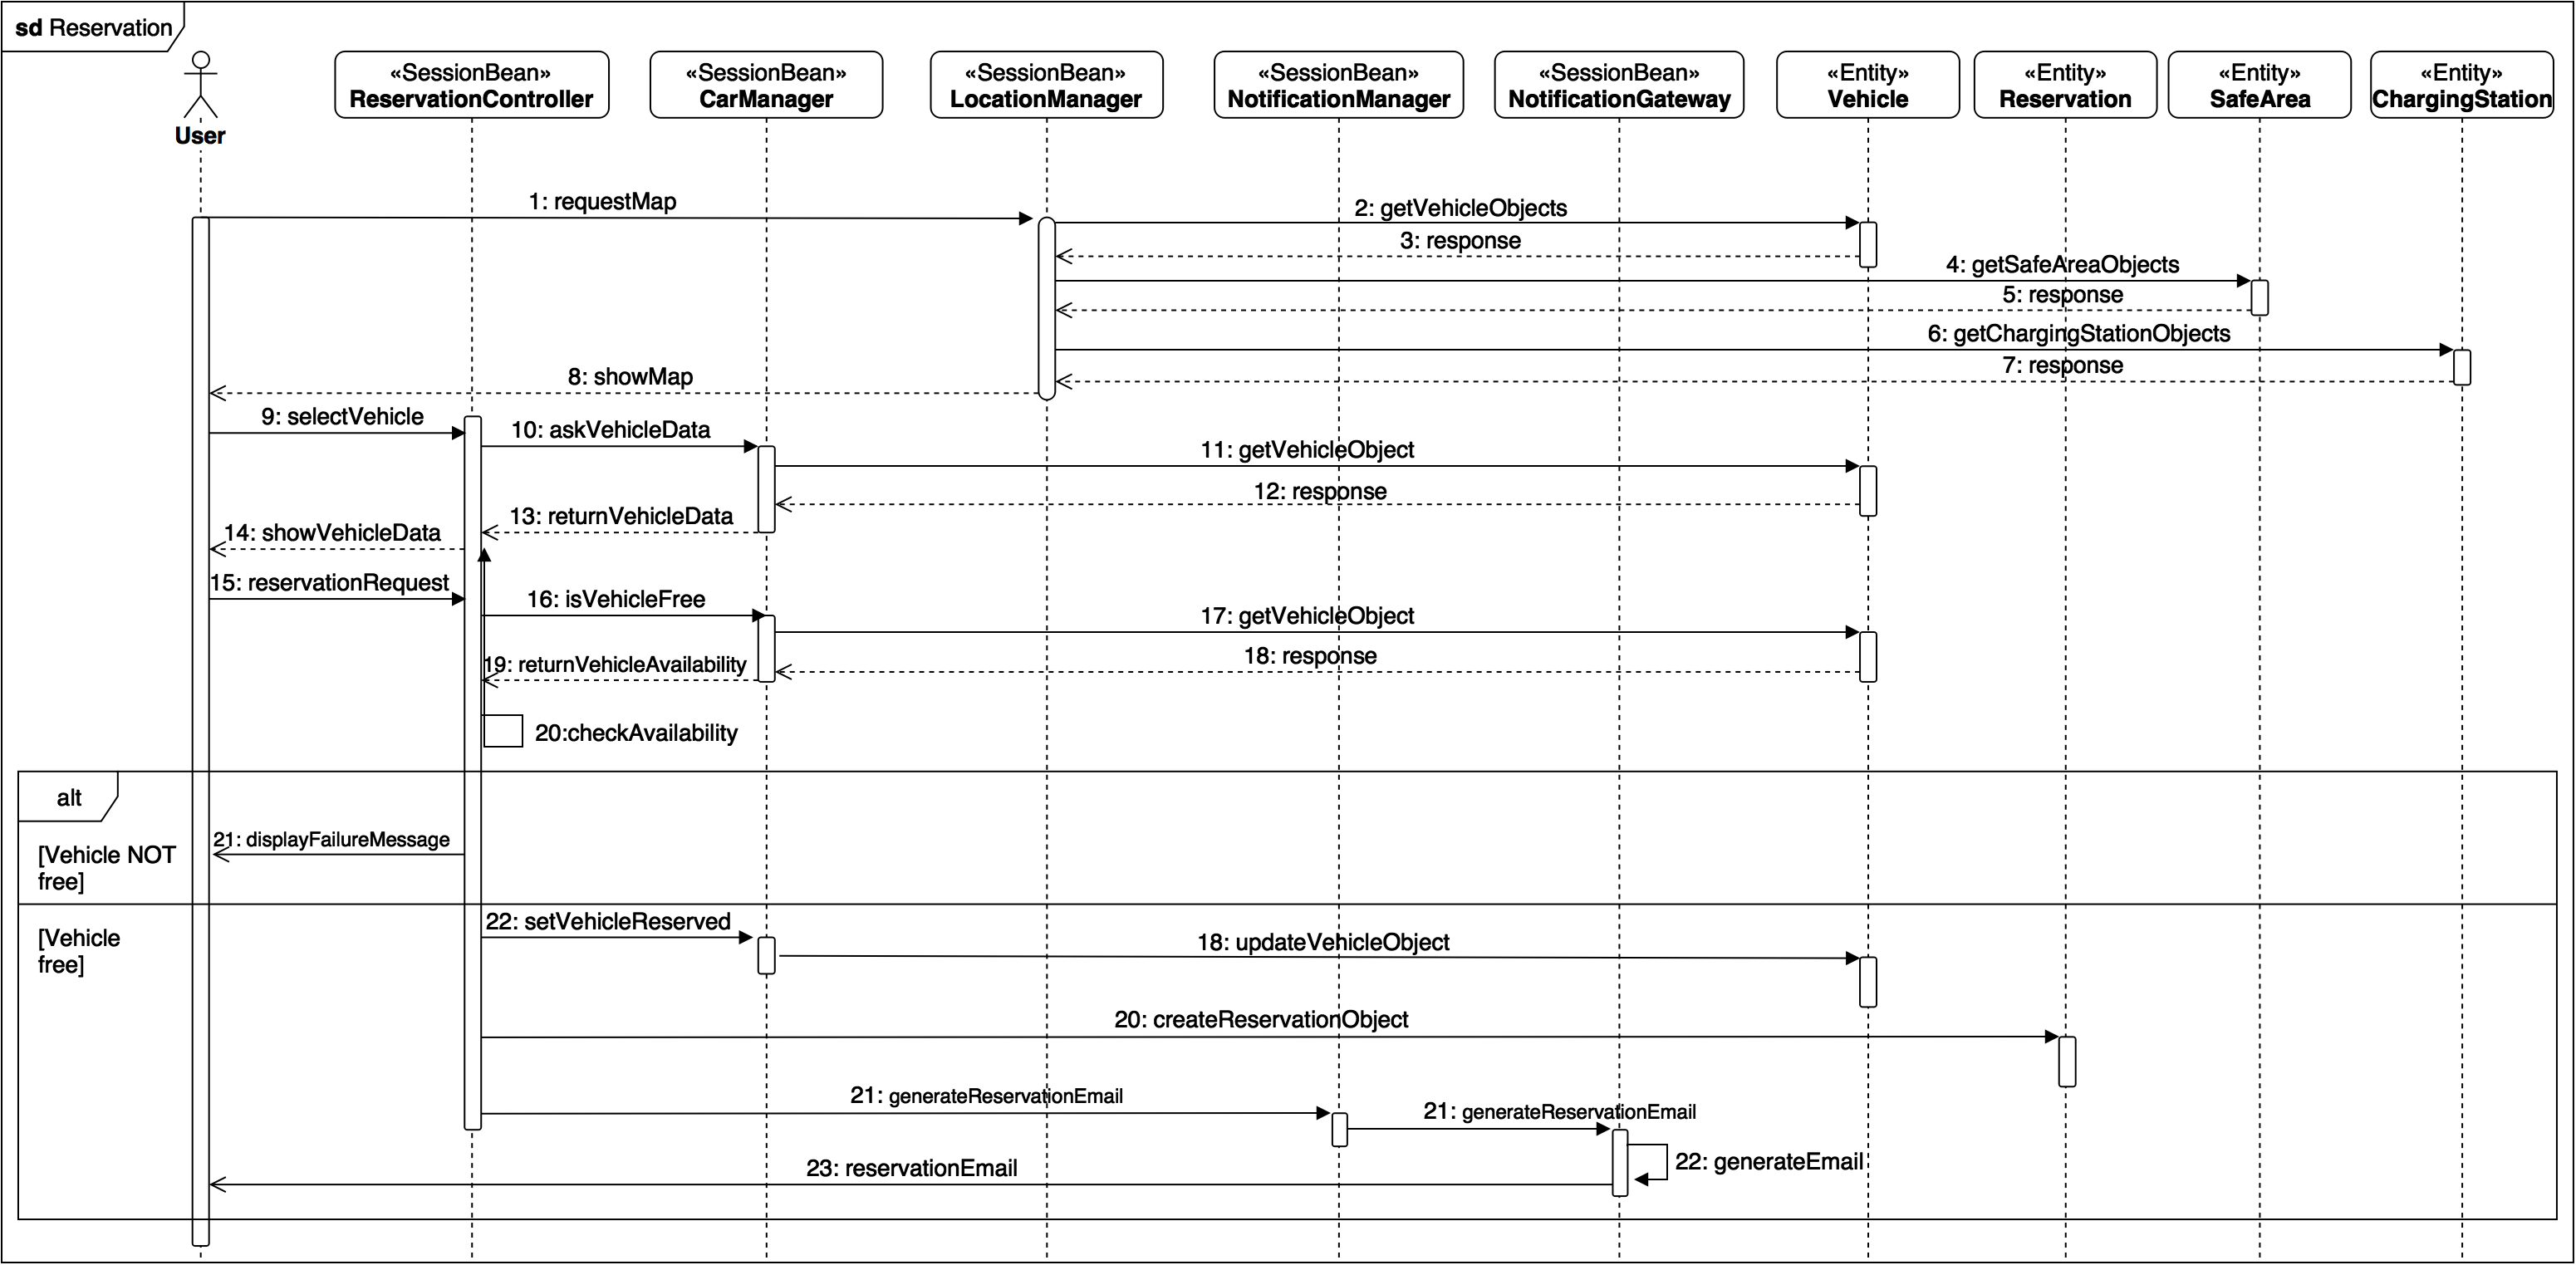
\includegraphics[width=1.0\textwidth]{/DD/Runtime_reservation}\\
  \vspace{0.4cm}
  \caption{Reservation sequence diagram: an user reserves a vehicle using the Mobile application. } 
  \label{fig:Runtime_reservation} 
\end{figure}
\newpage
\begin{figure}[!ht]
  \centering
  \vspace{0.2cm}
  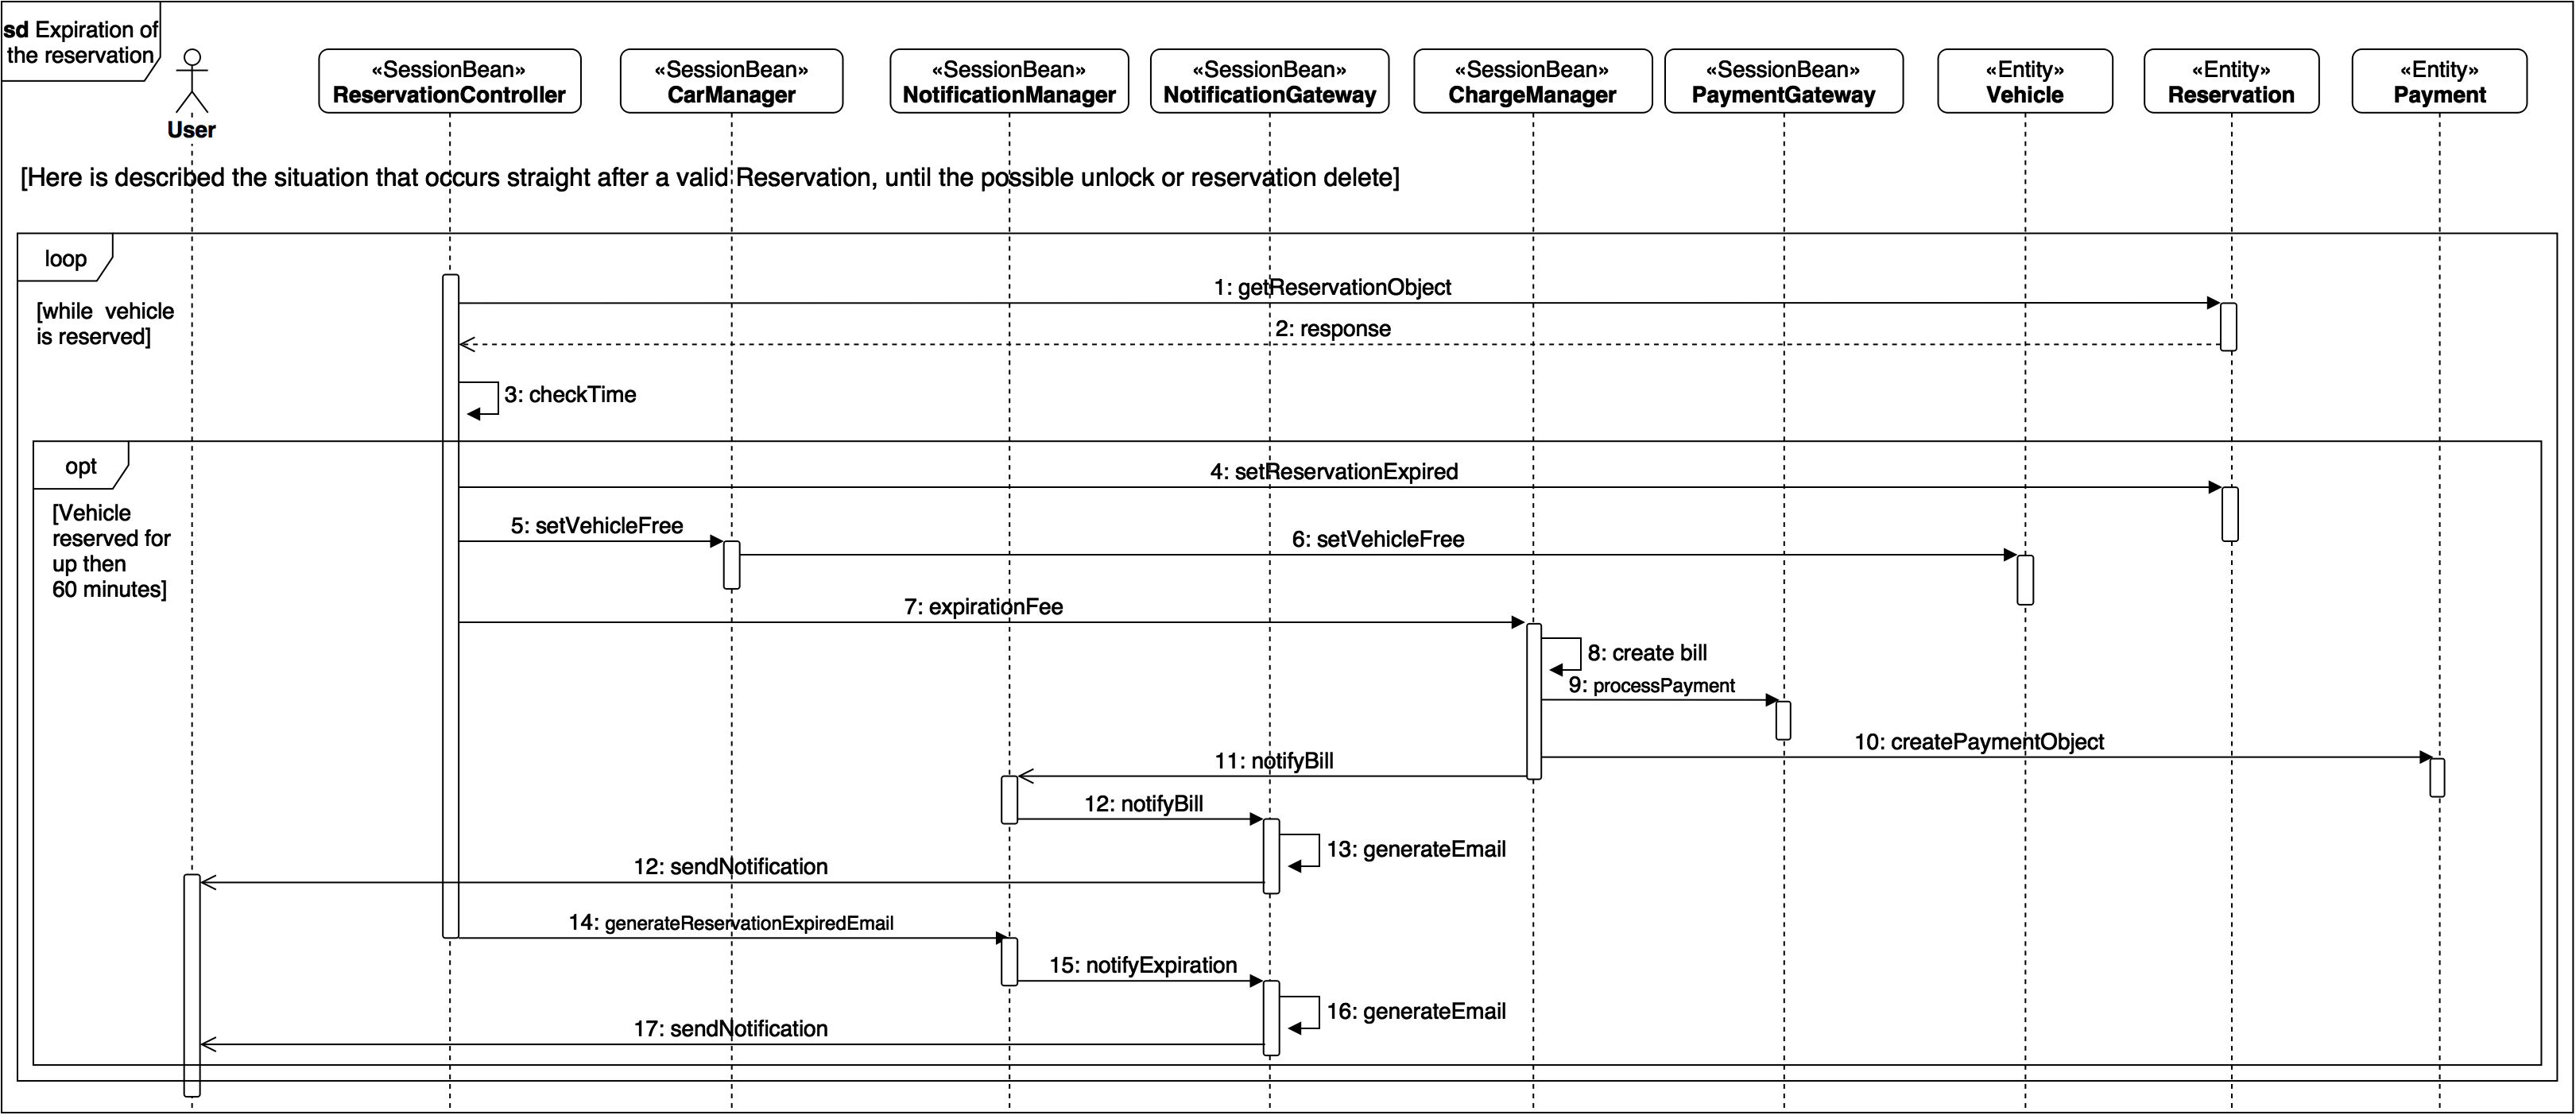
\includegraphics[width=1.0\textwidth]{/DD/Runtime_Expiration}\\
  \vspace{0.4cm}
  \caption{Expiration of the reservation sequence diagram: an user's reservation expires after an hour. The vehicle is tag FREE again. } 
  \label{fig:Runtime_Expiration} 
\end{figure}
\newpage
\begin{figure}[!ht]
  \centering
  \vspace{0.2cm}
  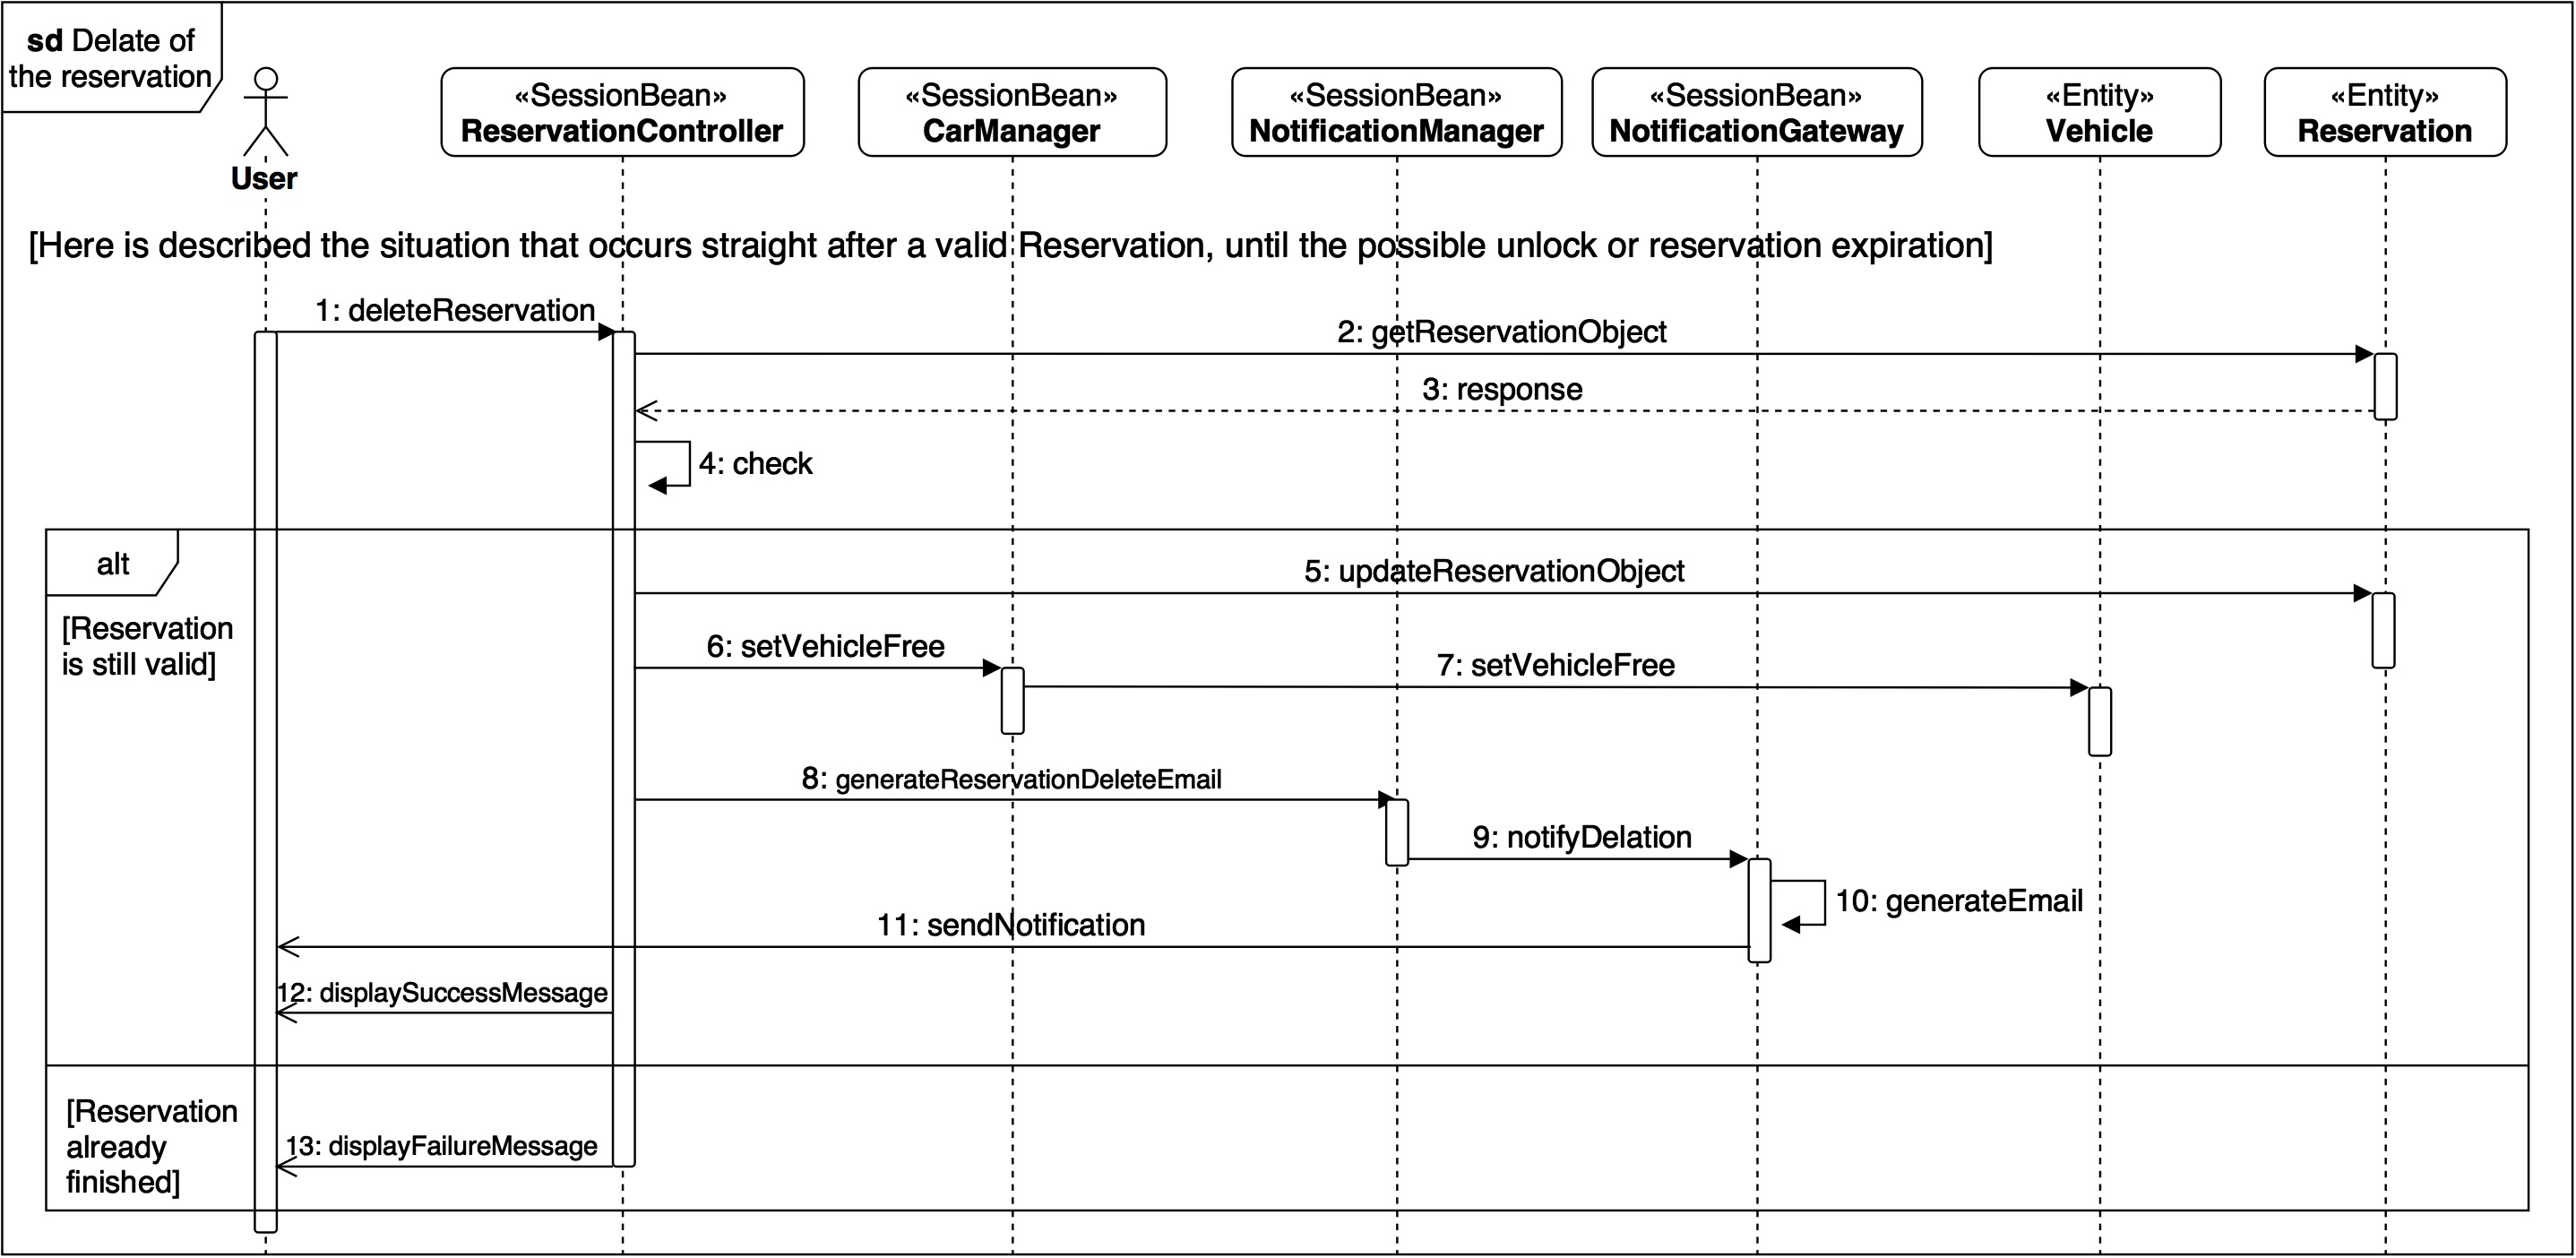
\includegraphics[width=1.0\textwidth]{/DD/Runtime_Delete_Reservation}\\
  \vspace{0.4cm}
  \caption{Deletion of the reservation sequence diagram: an user deletes her reservation. The vehicle is tag FREE again. } 
  \label{fig:Runtime_Delete_Reservation} 
\end{figure}
\newpage